In this Section, the current implementation is first compared with the one from Faney \sidecite{faney_spatially_2015} to ensure the additional assumptions do not produce different results.
A standard half-slab case is then described and a parametric study is performed by varying the exposure conditions.
Finally, the model is compared against experimental data.

\subsection{Tendril case} \labsec{tendril case}

\begin{figure*}
    \centering
    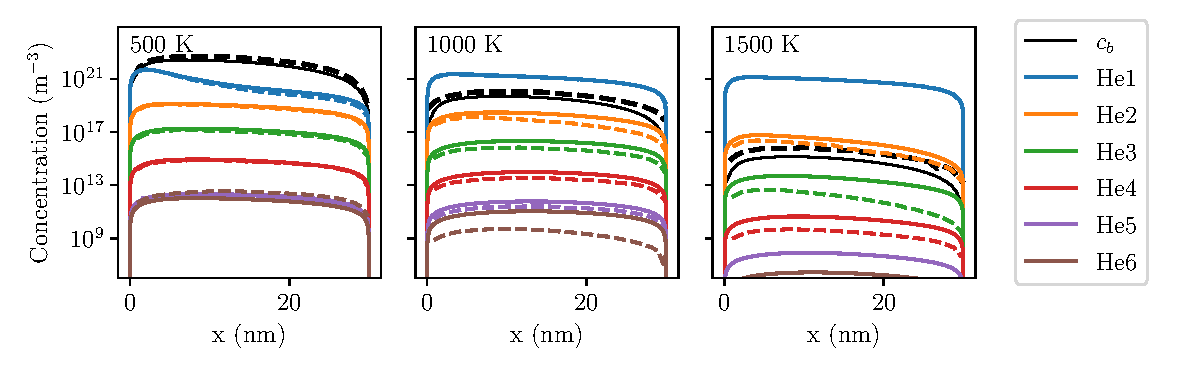
\includegraphics[width=\linewidth]{Figures/Chapter4/profiles_tendrils.pdf}
    \caption{He clusters concentration profiles in the tendril at \SI{500}{K}, \SI{1000}{K} and \SI{1500}{K}. Comparison between the current implementation (solid) and Faney's results \cite{faney_spatially_2015} (dashed).  Discrepancies at high temperature are likely due to the use of a different set of dissociation energies. At \SI{1000}{K} and \SI{1500}{K} the dashed and solid profiles of He$_1$ overlap.}
    \labfig{tendril profiles}
\end{figure*}

The tendril application case described in \cite{faney_spatially_2015} was simulated in 1D with the current implementation and the results were compared.

The domain size is \SI{30}{nm} and the volumetric source term is described as follows:
\begin{equation}
    \Gamma(x) = \varphi_\mathrm{imp} \; f(x) 
\end{equation}
where $\varphi_\mathrm{imp} = \SI{5e25}{m^{-2} s^{-1}}$ is the implanted He flux and $f(x)$ is a Gaussian distribution with a mean value $\mu = R_p = \SI{1.5}{nm}$ and a standard deviation $\sigma = \SI{1}{nm}$ which corresponds to a \SI{100}{eV} He implantation based on SRIM computations \sidecite{ziegler_srim_2010}.

Mobile He clusters concentrations were set to zero at the tendril's surfaces ($x=\SI{0}{nm}$ and $x=\SI{30}{nm}$).

Concentration profiles computed by the current implementation showed good agreement with the ones obtained by Faney et al \cite{faney_spatially_2015} (see \reffig{tendril profiles}).
The discrepancies are likely due to a difference in the set of dissociation energies that have been used.
Indeed, at low temperature, where dissociation is not activated, the discrepancies were very small whereas at high temperature, differences increased because dissociation became more dominant.
When $c_b$ is small compared to $c_{\mathrm{He}_1}$, the equilibrium of $\mathrm{He}_1$ is independent of these dissociation energies and the profiles for $\mathrm{He}_1$ are identical.

Moreover, increasing the temperature tended to inhibit bubble formation in the tendril.
This was explained by a greater increase in the dissociation rate and in losses at surfaces than the increase in the clustering rate.
This observation is in agreement with MD results simulating He implantation in tendrils \sidecite{wei_better_2020, wei_understanding_2019}.
The current implementation and the additional assumptions that were made are therefore valid.

\subsection{Half-slab case} \labsec{half slab}

\begin{figure}
    \centering
    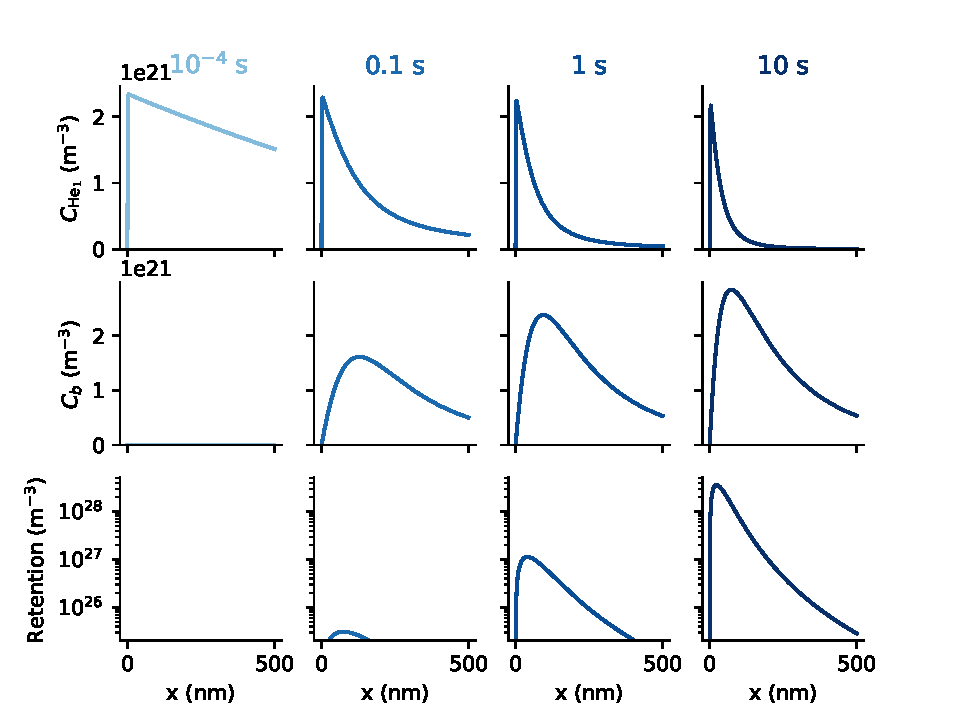
\includegraphics[width=\linewidth]{Figures/Chapter4/half_slab/profiles_half_slab.pdf}
    \caption{Concentration profiles of He$_1$ (left) and bubbles (right) in W exposed to \SI{100}{eV} He at \SI{e22}{m^{-2}.s^{-1}} and \SI{1000}{K}.}
    \labfig{profiles half slab}
\end{figure}

He transport was simulated in a 1D semi-infinite W slab.
This case is the standard case describing the main quantities of interest of the parametric study performed in \refsec{parametric study}.

The domain size is \SI{0.1}{mm} which is much greater than the penetration depth of He in the simulations.
\SI{100}{eV} He were implanted in the first \SI{1.5}{nm} as in \refsec{tendril case}.
The implanted flux was \SI{1e22}{m^{-2} s^{-1}} and the temperature was \SI{1000}{K}.

At low \glspl{fluence}, He diffused really quickly into the bulk (see \reffig{profiles half slab}) and the bubbles concentration $c_b$ was found to be zero.
As the \gls{fluence} increased, bubbles started to appear and acted as strong sinks for mobile He.
This lead to a great decrease in the mobile He concentration profile.

It is worth noticing the maximum of $c_b$ was not located at the maximum of $c_{\mathrm{He}_1}$ which is the implantation depth $R_p$.
This was explained by the diffusion of small mobile clusters as shown by analytical models \sidecite{krasheninnikov_helium_2014}.
As He clusters, small mobile clusters diffuse deeper into the bulk until \gls{trap mutation} occurs and bubbles nucleons (clusters with more than 6 He) are created.
From that point, bubbles are formed relatively far from the surface.
Because He is implanted in the first nanometres, $c_{\mathrm{He}_1}$ is maximum at $R_p = \SI{1.5}{nm}$ and interactions with bubbles are stronger in this region.
This tends to draw the maximum location of $c_b$ towards the surface.

The He content in bubbles $\langle i_b \rangle$ and the radius $\langle r_b \rangle$ were computed.
After \SI{10}{s} of implantation, bubbles located in the near surface contained up to \SI{3e7}{He}.
The maximum of $\langle r_b \rangle$ was found to be very close to the surface at approximately \SI{2}{nm} (see \reffig{profiles rb half slab}).
This is explained by the high concentration of mobile He in this near surface region.
Moreover, a bursting zone can be defined by the region where $\langle r_b \rangle$ is greater than the depth of the bubble.
In this region, bubble of this size would have likely burst.
% This result was in good agreement with the He bubbles observations performed by Ialovega \textit{et al} on W \sidecite{ialovega_hydrogen_2020}.

\begin{figure} [h]
    \centering
    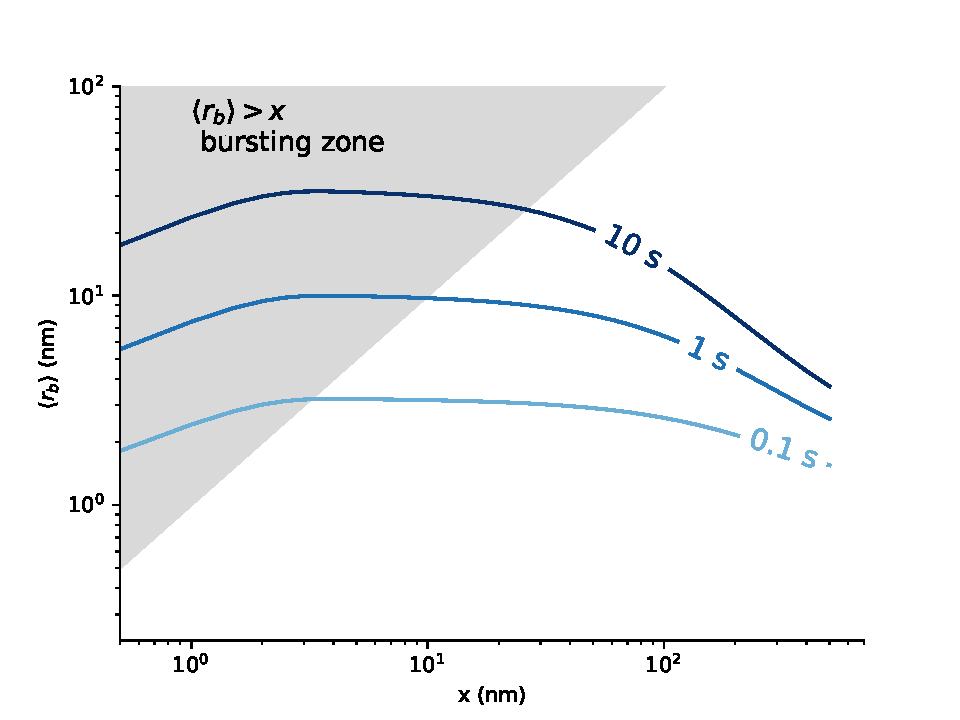
\includegraphics[width=\linewidth]{Figures/Chapter4/half_slab/profile_rb.pdf}
    \caption{Profile of mean bubble radius $\langle r_b \rangle$ as a function of depth $x$ in W exposed to \SI{100}{eV} He at \SI{e22}{m^{-2}.s^{-1}} and \SI{1000}{K}.}
    \labfig{profiles rb half slab}
\end{figure}

\begin{figure*}
    \centering
    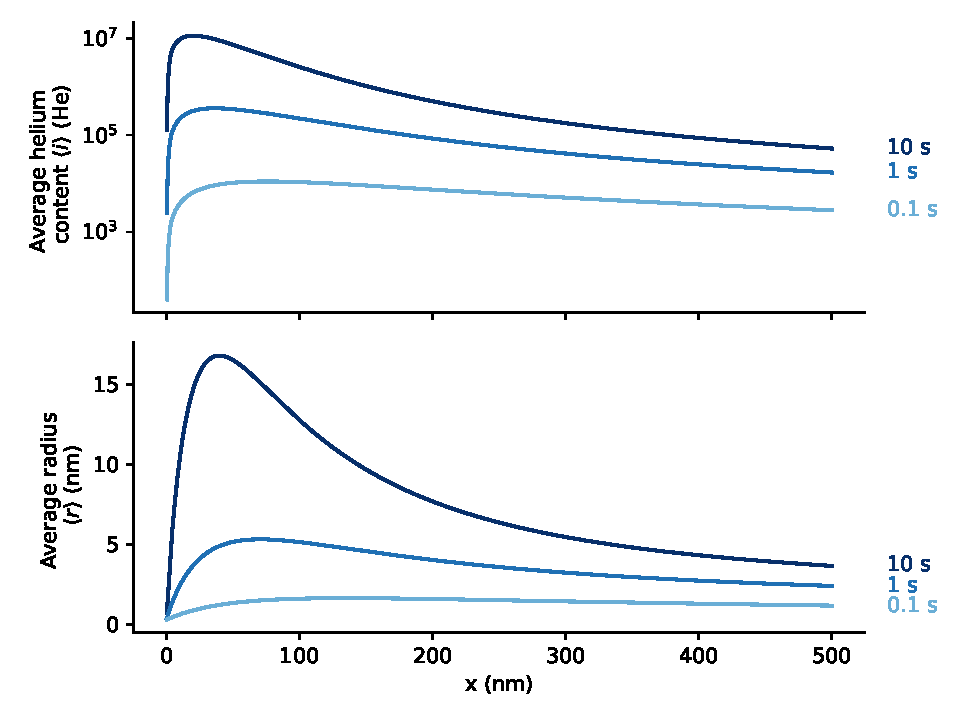
\includegraphics[width=0.75\linewidth]{Figures/Chapter4/half_slab/average_content_radius.pdf}
    \caption{Average helium content $\langle i \rangle$ and average radius $\langle r \rangle$ in all clusters (mobile and bubbles) in W exposed to \SI{100}{eV} He at \SI{e22}{m^{-2}.s^{-1}} and \SI{1000}{K}.}
    \labfig{content and radius}
\end{figure*}

From this average He content in bubbles and from Equations \refeq{radius average} and \refeq{radius pure He} expressing the clusters radii, the average radius $\langle r \rangle$ can be computed as:

\begin{equation}
        \langle r \rangle = \frac{\sum\limits_{i=1}^\infty c_i r_i}{\sum\limits_{i=1}^\infty c_i}
        = \frac{\sum\limits_{i=1}^N c_i r_i + c_b \langle r_b \rangle }{\sum\limits_{i=1}^N c_i + c_b}
\end{equation}

The average content of He in all clusters $\langle i \rangle$ is computed in a similar way:
\begin{equation}
        \langle i \rangle = \frac{\sum\limits_{i=1}^\infty c_i i}{\sum\limits_{i=1}^\infty c_i}
        = \frac{\sum\limits_{i=1}^N c_i i + c_b \langle i_b \rangle }{\sum\limits_{i=1}^N c_i + c_b}
\end{equation}

These two quantities are comparable to the ones obtained by Faney \textit{et al} \sidecite{faney_spatially_2015}.
After \SI{100}{s} of exposure, the average radius \SI{50}{nm} below the surface was above \SI{10}{nm} (see \reffig{content and radius}).
Moreover, the location of the maximum of these quantities move towards the exposed surface.

The average radius $\langle r \rangle$ cannot be easily compared to experimental observations for it includes contributions from very small mobile He$_x$ clusters which are not visible experimentally (only bubbles with a radius greater than 1-\SI{3}{nm} are observable depending on the observation technique).

\subsection{Influence of exposure parameters on He bubble growth}
The impact of He flux and temperature $T$ was studied on the case described in \refsec{half slab} in order to identify trends.
Behaviour laws are identified and can be used to obtain information on He transport without needing to run any simulation.

\subsubsection{Parametric study} \labsec{parametric study}

\begin{figure*} [ht!]
    \centering
    \begin{subfigure}{0.5\linewidth}
        \centering
        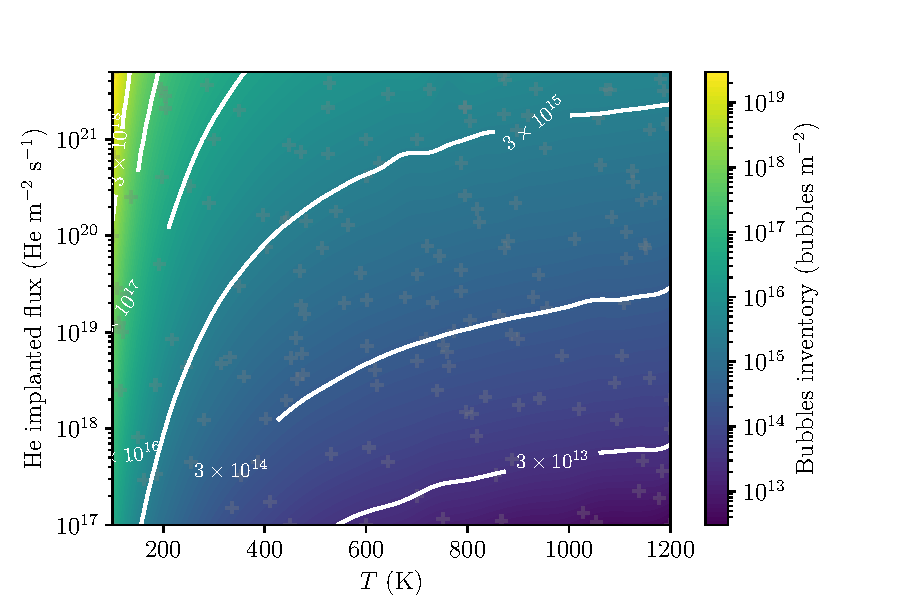
\includegraphics[width=\linewidth]{Figures/Chapter4/parametric study/bubbles_total_T_phi.pdf}
        \caption{Bubbles inventory $I_b = \int c_b \; dx$.}
        \labfig{inventory bubbles T phi}
    \end{subfigure}%
    \begin{subfigure}{0.5\linewidth}
        \centering
        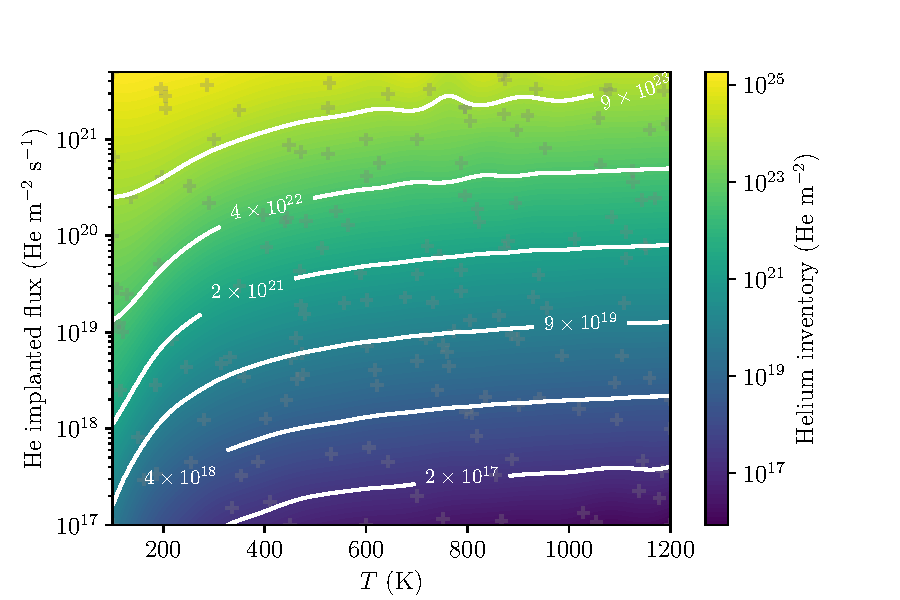
\includegraphics[width=\linewidth]{Figures/Chapter4/parametric study/inventory_T_phi.pdf}
        \caption{He inventory $I = \int \langle i_b \rangle c_b \; dx$.}
        \labfig{He inventory T phi}
    \end{subfigure}
    % \begin{subfigure}{0.5\linewidth}
    %     \centering
    %     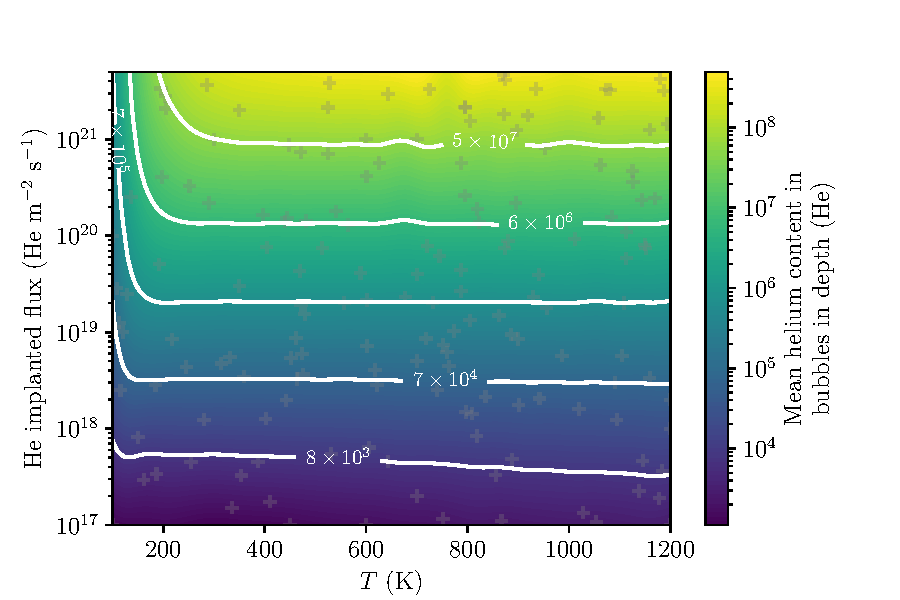
\includegraphics[width=\linewidth]{Figures/Chapter4/parametric study/mean_ib_T_phi.pdf}
    %     \caption{mean $\langle i_b \rangle$}
    % \end{subfigure}%
    % \begin{subfigure}{0.5\linewidth}
    %     \centering
    %     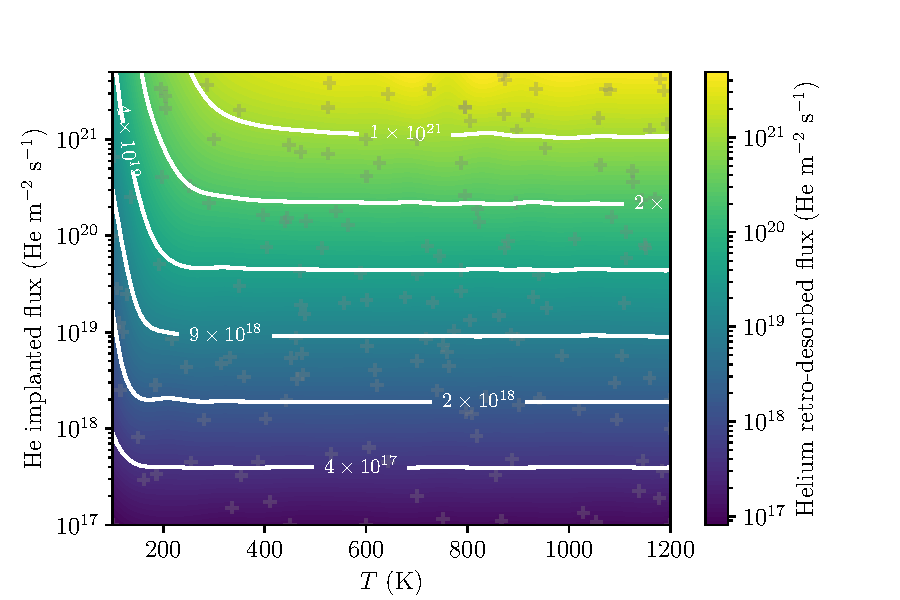
\includegraphics[width=\linewidth]{Figures/Chapter4/parametric study/surface_flux_T_phi.pdf}
    %     \caption{Retrodesorbed flux}
    % \end{subfigure}
    \begin{subfigure}{0.5\linewidth}
        \centering
        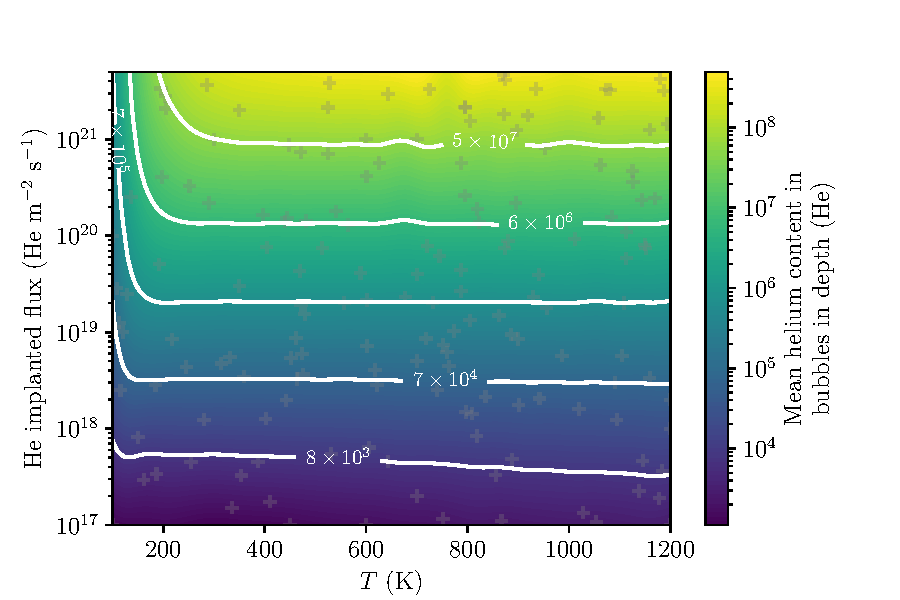
\includegraphics[width=\linewidth]{Figures/Chapter4/parametric study/mean_ib_T_phi.pdf}
        \caption{Average He content in bubbles $\Bar{\langle i_b \rangle} = I / I_b$.}
        \labfig{mean ib T phi}
    \end{subfigure}%
    \begin{subfigure}{0.5\linewidth}
        \centering
        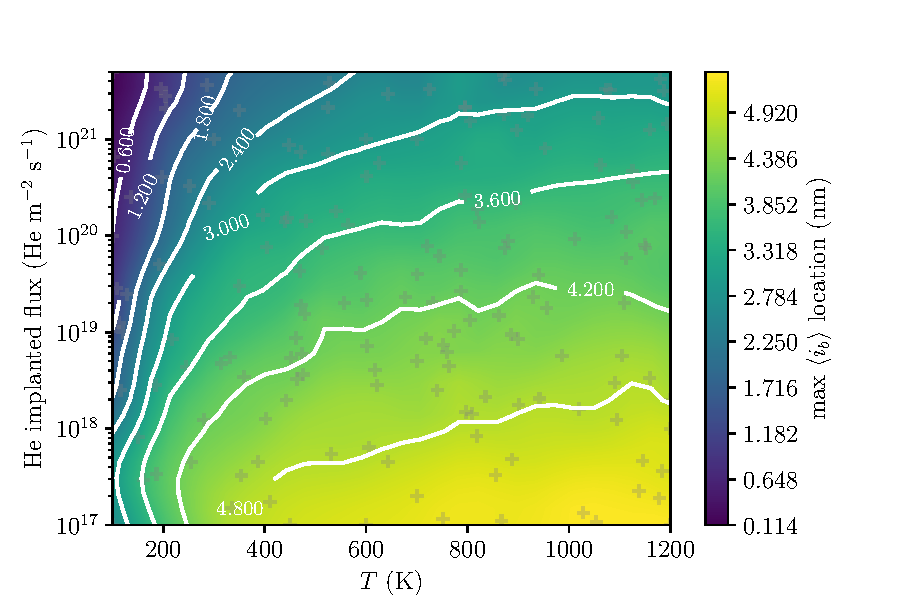
\includegraphics[width=\linewidth]{Figures/Chapter4/parametric study/x_max_ib_T_phi.pdf}
        \caption{Location of max $\langle i_b \rangle$.}
        \labfig{x max ib T phi}
    \end{subfigure}
    \caption{Evolution of quantities as a function of the implanted flux and temperature after \SI{1}{h} of \SI{100}{eV} He exposure. Grey crosses correspond to simulations points.}
    \labfig{T phi quantities}
\end{figure*}

A parametric study was performed by varying the implanted flux $\varphi_\mathrm{imp}$ between \SI{1e17}{m^{-2} s^{-1}} and \SI{5e21}{m^{-2} s^{-1}} and the sample temperature $T$ between \SI{100}{K} and \SI{1200}{K}.

Several quantities were computed.
First the bubbles inventory is defined as:
\begin{equation}
    I_\mathrm{bubbles}= \displaystyle \int c_b \; dx
\end{equation}
The total helium inventory is calculated by:
\begin{equation}
        I = \displaystyle \int \sum\limits_{i=1}^N i c_i + \langle i_b \rangle c_b \; dx
        \approx \displaystyle \int \langle i_b \rangle c_b \; dx
    \labeq{I}
\end{equation}
The spatial mean helium content in bubbles can be computed as:
\begin{equation}
        \Bar{\langle i_b \rangle} = \frac{\displaystyle \int \langle i_b \rangle c_b \; dx}{\displaystyle \int c_b \; dx}
        \approx \frac{I}{I_\mathrm{bubbles}}
    \labeq{mean ib}
\end{equation}
The approximation made in Equations \refeq{I} and \refeq{mean ib} is valid as long as $\int \langle i_b \rangle c_b dx \gg  \int \sum\limits_{i=1}^N i c_i dx$ (\textit{ie} the He inventory is dominated by that of the bubbles).
This is the case in these simulations because $N=6$ (the influence of this parameter is discussed in \refsec{impact of N}).

More than 160 simulations were performed simulating \SI{1}{h} of exposure.
For each simulation, the quantities of interest described above were computed.
A Gaussian regression process \sidecite{chris_bowman_c-bowmaninference-tools_2020} was used to interpolate the data based on Bayesian inference as done in \sidecite{delaporte-mathurin_parametric_2020} (see \reffig{T phi quantities}).
The temporal evolution of these quantities was also assessed (see \reffig{quantities time}).

% bubbles inventory
After \SI{1}{h} of exposure, the bubbles inventory $I_\mathrm{bubbles}$ shows a weak dependence on temperature at high temperature and a weak dependence on the implanted flux at low temperature (see \reffig{inventory bubbles T phi}).
$I_\mathrm{bubbles}$ varies from \SI{4e12}{\text{bubbles } m^{-2}} at high temperature and low flux to \SI{2e19}{\text{bubbles } m^{-2}} at low temperature and high flux.

% He inventory
The He inventory $I$ varies from \SI{8e16}{m^{-2}} at high temperature and low flux to \SI{e25}{m^{-2}} at low temperature and high flux (see \reffig{He inventory T phi}).
For temperatures above \SI{600}{K}, the temperature dependence is rather weak compared to the flux dependence.

% mean ib
For temperatures above \SI{300}{K}, and after \SI{1}{h} of exposure, the sample temperature does not impact the value of $\Bar{\langle i_b \rangle}$ (see \reffig{mean ib T phi}).
The mean He content increases with the implanted flux as expected and varies between \SI{e3}{He} at low flux and \SI{5e8}{He} at high flux.

% x max ib
The position of the maximum of $\langle i_b \rangle$ tended to increase with temperature and decrease with implanted flux (see \reffig{x max ib T phi}).
After \SI{1}{h} of exposure, it was found to be really close to the surface down to \SI{0.1}{nm} at low temperatures and high fluxes.
The validity of the model in this region of the parameter space is questionable considering that the bubble radius is greater that the thickness of the ligament between the edge of the bubble and the surface.
Such a bubble would therefore have burst before reaching this size. 

\begin{figure*} [ht!]
    \centering
    \begin{subfigure}{0.5\linewidth}
        \centering
        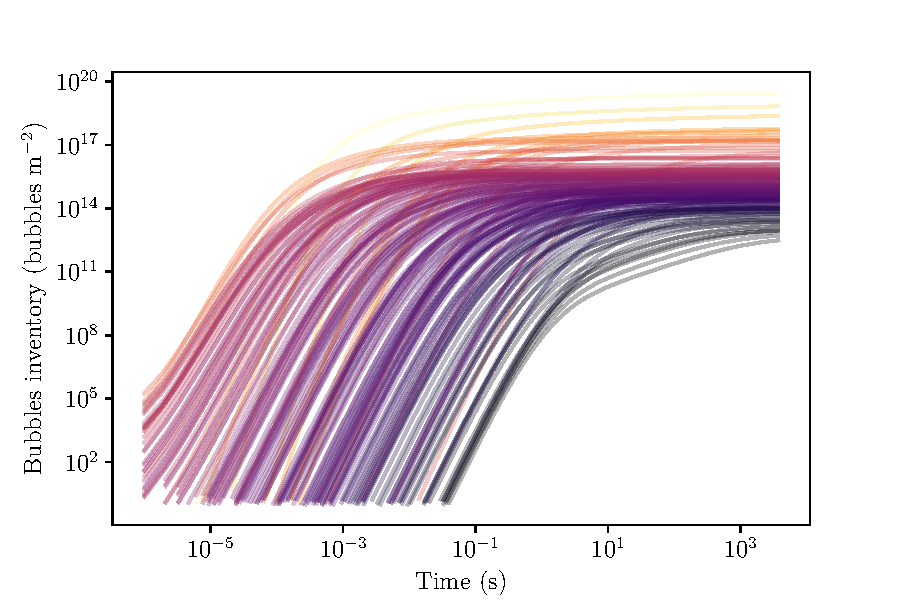
\includegraphics[width=\linewidth]{Figures/Chapter4/parametric study/total_bubbles_time.pdf}
        \caption{Bubbles inventory $I_b = \int c_b \; dx$.}
        \labfig{inventory bubbles time}
    \end{subfigure}%
    \begin{subfigure}{0.5\linewidth}
        \centering
        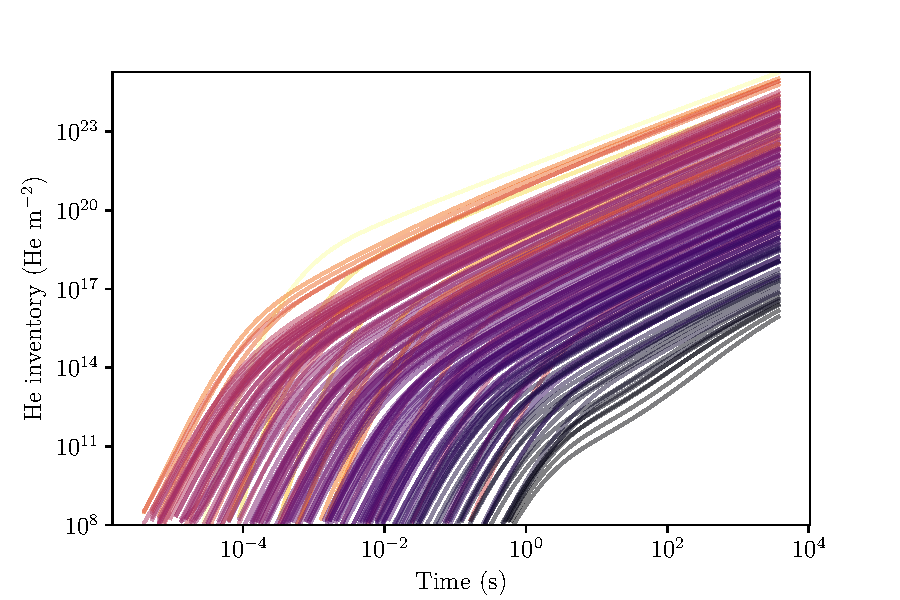
\includegraphics[width=\linewidth]{Figures/Chapter4/parametric study/inventory_time.pdf}
        \caption{He inventory $I = \int \langle i_b \rangle c_b \; dx$.}
        \labfig{He inventory time}
    \end{subfigure}
    % \begin{subfigure}{0.5\linewidth}
    %     \centering
    %     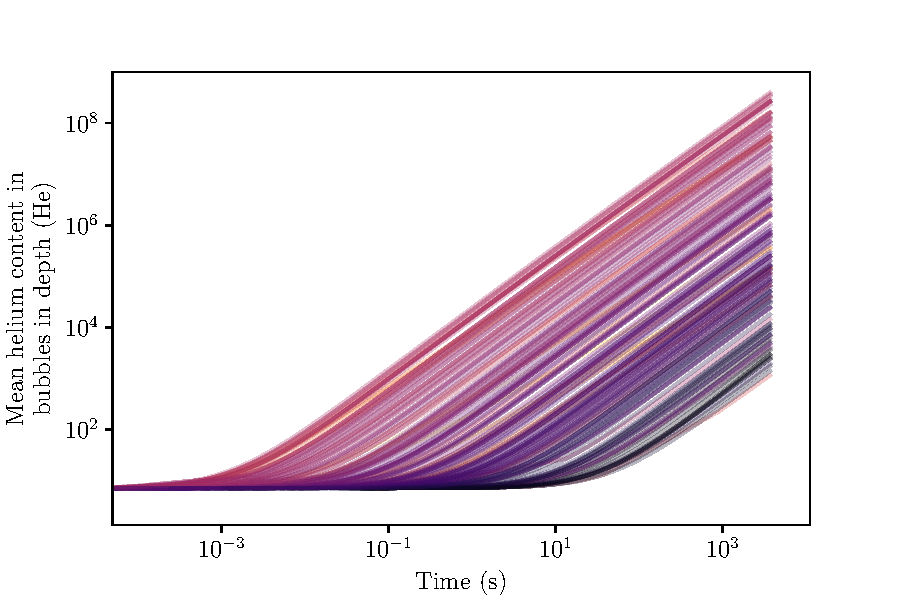
\includegraphics[width=\linewidth]{Figures/Chapter4/parametric study/mean_ib_time.pdf}
    %     \caption{mean $\langle i_b \rangle$}
    % \end{subfigure}%
    % \begin{subfigure}{0.5\linewidth}
    %     \centering
    %     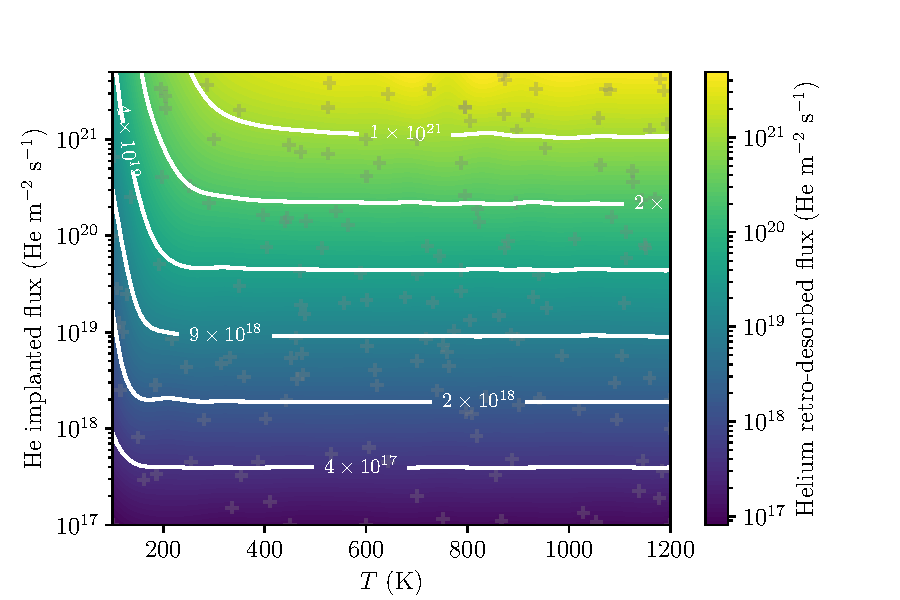
\includegraphics[width=\linewidth]{Figures/Chapter4/parametric study/surface_flux_T_phi.pdf}
    %     \caption{Retrodesorbed flux}
    % \end{subfigure}
    \begin{subfigure}{0.5\linewidth}
        \centering
        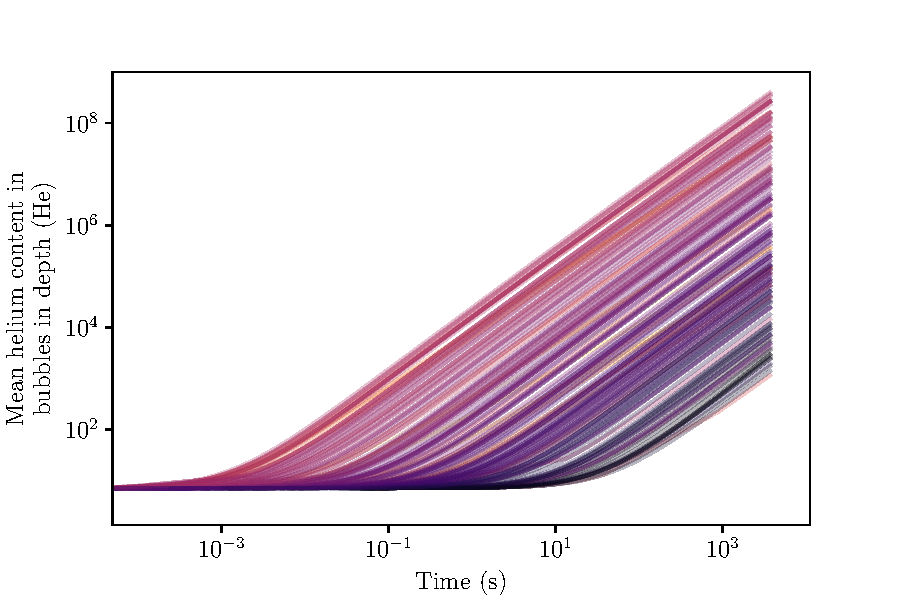
\includegraphics[width=\linewidth]{Figures/Chapter4/parametric study/mean_ib_time.pdf}
        \caption{Average He content in bubbles $\Bar{\langle i_b \rangle} = I / I_b$.}
        \labfig{mean ib time}
    \end{subfigure}%
    % \begin{subfigure}{0.5\linewidth}
    %     \centering
    %     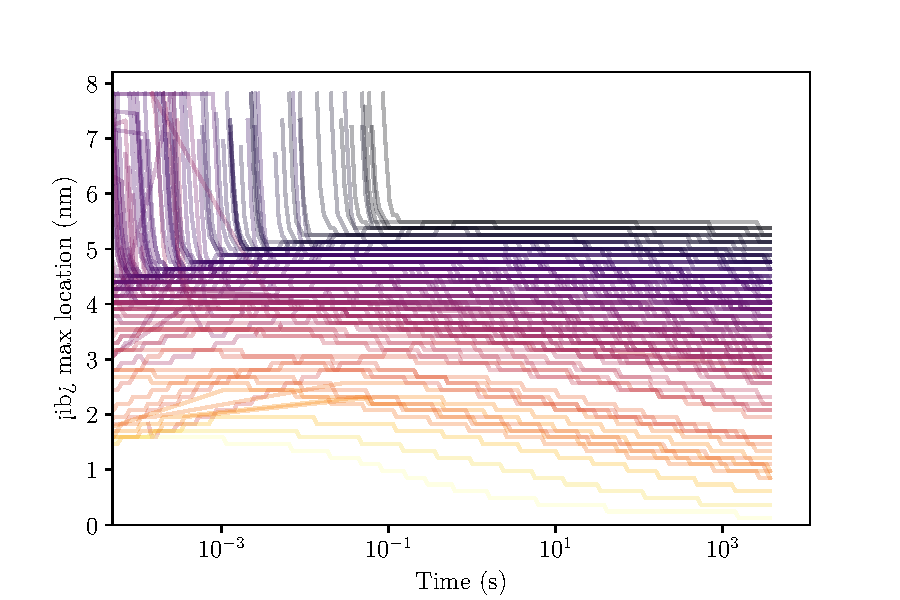
\includegraphics[width=\linewidth]{Figures/Chapter4/parametric study/x_max_ib_time.pdf}
    %     \caption{x max $\langle i_b \rangle$}
    %     \labfig{x max ib time}
    % \end{subfigure}
    \begin{subfigure}{0.5\linewidth}
        \centering
        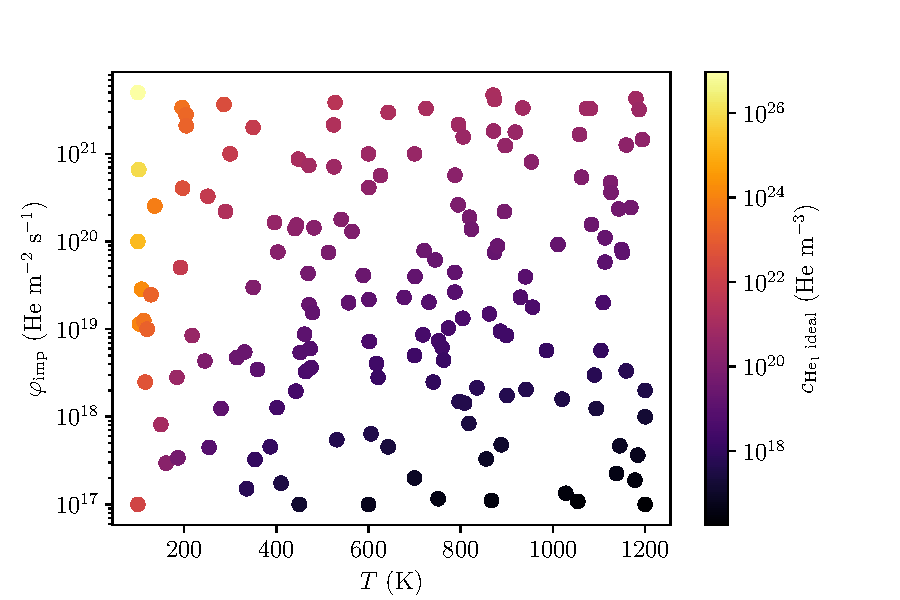
\includegraphics[width=\linewidth]{Figures/Chapter4/parametric study/points_with_parameter.pdf}
        \caption{Simulation points coloured according to $c_{\mathrm{He}_1, \mathrm{ideal}}$.}
        \labfig{simulations points with parameter}
    \end{subfigure}
    \caption{Temporal evolution of quantities in W exposed to \SI{100}{eV} He at \SI{e22}{m^{-2}.s^{-1}} and \SI{1000}{K} for temperatures varying from \SI{120}{K} to \SI{1200}{K} and implanted fluxes varying from \SI{e17}{m^{-2}s^{-1}} to \SI{e21}{m^{-2}s^{-1}}. Each line corresponds to a simulation point (grey crosses on \reffig{inventory bubbles T phi} and points on \reffig{simulations points with parameter}). The lines are coloured according to the parameter $c_{\mathrm{He}_1, \mathrm{ideal}} = \varphi_\mathrm{imp} \; R_p/D(T)$ with $R_p = \SI{1.5}{nm}$ and $D$ the diffusion coefficient of $\mathrm{He}_1$ in W.}
    \labfig{quantities time}
\end{figure*}

% time series
For each simulation point, the temporal evolution of the quantities described above has been computed.
To better identify the time series on the $\varphi_\mathrm{imp}, T$ plane, lines have been coloured according to the parameter $c_{\mathrm{He}_1, \mathrm{ideal}}$ which is a function of both the implanted flux and the temperature (see Equation \refeq{c he1 ideal}) expressed in \si{m ^{-3}}.

\begin{equation}
    c_{\mathrm{He}_1, \mathrm{ideal}} = \frac{\varphi_\mathrm{imp} \; R_p}{D(T)}
    \labeq{c he1 ideal}
\end{equation}
where $\varphi_\mathrm{imp}$ is the implanted flux, $D$ is the diffusion coefficient of mobile $\mathrm{He}_1$ in W (see \reftab{clusters properties}), $R_p = \SI{1.5}{nm}$ is the implantation depth and $T$ is the temperature in \si{K}.

All these quantities showed a similar behaviour in time even though the kinetics were found to be different (see \reffig{quantities time}).
For instance, for each $(T, \varphi_\mathrm{imp})$ couple, $I_\mathrm{bubbles}$ first increased as a power law of time before reaching a maximum (see \reffig{inventory bubbles time}).
The total He inventory $I$ increased with time and for each simulation point but the growth rate decreased at long exposure times (see \reffig{He inventory time}).
This phenomenon is explained in details in \refsec{nucleation growth phases}.
Similarly, $\Bar{\langle i_b \rangle}$ could be written as a power law of time described in Eq \refeq{ib evolution} (see \reffig{mean ib time}).
The depth of the maximum of $\langle i_b \rangle$ tended to decrease with time as it was observed in \refsec{half slab} (see \reffig{inventory bubbles time}).

\subsubsection{Identification of regimes for inventory evolution} \labsec{nucleation growth phases}

\begin{figure} [h]
    \centering
    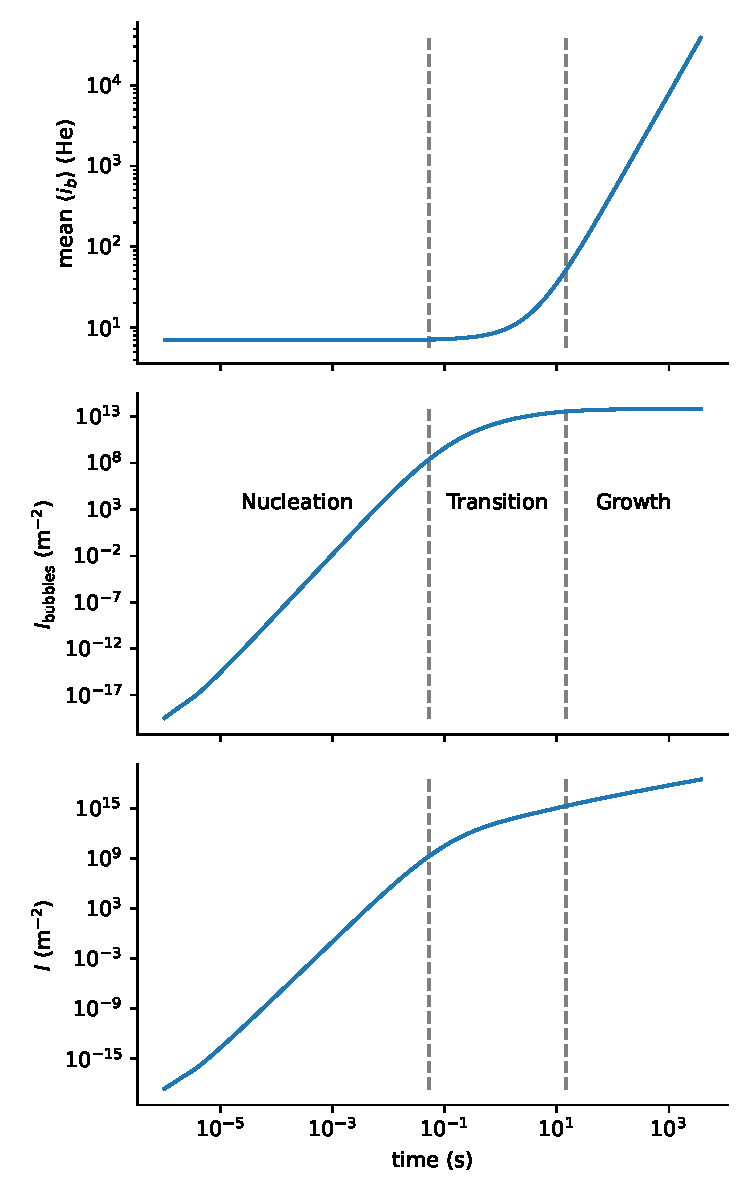
\includegraphics[width=0.75\linewidth]{Figures/Chapter4/parametric study/inventory_bubbles_ib.pdf}
    \caption{Temporal evolution of $\Bar{\langle i_b \rangle}$, $I_\mathrm{bubbles}$ and $I$ in W exposed to \SI{100}{eV} He at \SI{1.59e18}{m^{-2}.s^{-1}} and \SI{1020}{K}. The dashed grey vertical line represents the transition from nucleation regime to bubble growth regime.}
    \labfig{two regimes}
\end{figure}

For every $(T, \varphi_\mathrm{imp})$ couple, $I_\mathrm{bubbles}$ increased rapidly at low \glspl{fluence} until reaching a maximum at high \glspl{fluence} (see \reffig{inventory bubbles time}).
On the other hand, the mean He content $\Bar{\langle i_b \rangle}$ was constant at low \glspl{fluence} and increased as a power law of time at high \glspl{fluence} (see \reffig{mean ib time}).
The evolution of $\Bar{\langle i_b \rangle}$ can be described as:
\begin{equation}
    \Bar{\langle i_b \rangle} = N + 1 + a \; t^b
    \labeq{ib evolution}
\end{equation}
where $N=6$ in this model, $a$ and $b$ depend on $(T, \varphi_\mathrm{imp})$.
The choice of $N=6$ in this model is detailed in \refsec{impact of N}.
The total He inventory $I$ being the product of these two quantities, two different growth rates were observed (see \reffig{He inventory time} and \reffig{two regimes}).

This phenomenon can be attributed to two different regimes.
The first regime is the nucleation regime where new bubbles nucleons are created (\textit{ie} $c_b$ and $I_\mathrm{bubbles}$ increase).
In the nucleation regime, the bubble concentration $c_b$ and the capture radius $\langle r_b \rangle$ are too low for the He content in bubbles $\langle i_b \rangle$ to increase significantly (\textit{ie} $\Bar{\langle i_b \rangle}$ is constant).
The second regime is the bubble growth regime.
In this regime, $c_b$ is high enough for interactions between bubbles and mobile He to occur.
Implanted interstitial He atoms ($c_{\mathrm{He}_1}$) therefore interact preferably with bubbles rather than clustering with other interstitial He atoms.
This means that no additional bubbles nucleons are created (\textit{ie} $c_b$ reaches a maximum).
Because interactions between bubbles and mobile He are strong, the term $\langle k_b^+ \rangle c_1 c_b$ in Equation \refeq{temporal evolution grouping} becomes significant and the He content increases (\textit{ie} $\Bar{\langle i_b \rangle}$ increases).
This is illustrated by the thickness of the interaction arrows in \reffig{clustering sketch}.


\subsubsection{Influence of $N$} \labsec{impact of N}
In order to assess the impact of the parameter $N$ in Equation \refeq{temporal evolution grouping}, the evolution of the He inventory $I$, the mean He content in immobile clusters (different from $\Bar{\langle i_b \rangle}$) and the bubbles inventory $I_\mathrm{bubbles}$ was computed with several values of $N$.

The flux of \SI{100}{eV} He in this test case was \SI{e20}{m^{-2} s^{-1}} and the temperature was \SI{1000}{K}. 

It was shown that varying $N$ had no impact on these quantities whatsoever (see \reffig{N variation}).
This highlights the very quick transition from nucleation regime to growth regime in this model.

The number of equations that need to be solved can therefore be minimised by setting the parameter $N$ to its minimum ($N=6$) without losing accuracy in the results.
This minimum value corresponds to the number of mobile clusters which have to be explicitly simulated in order to account for all the diffusion mechanisms.

\begin{figure} [h]
    \centering
    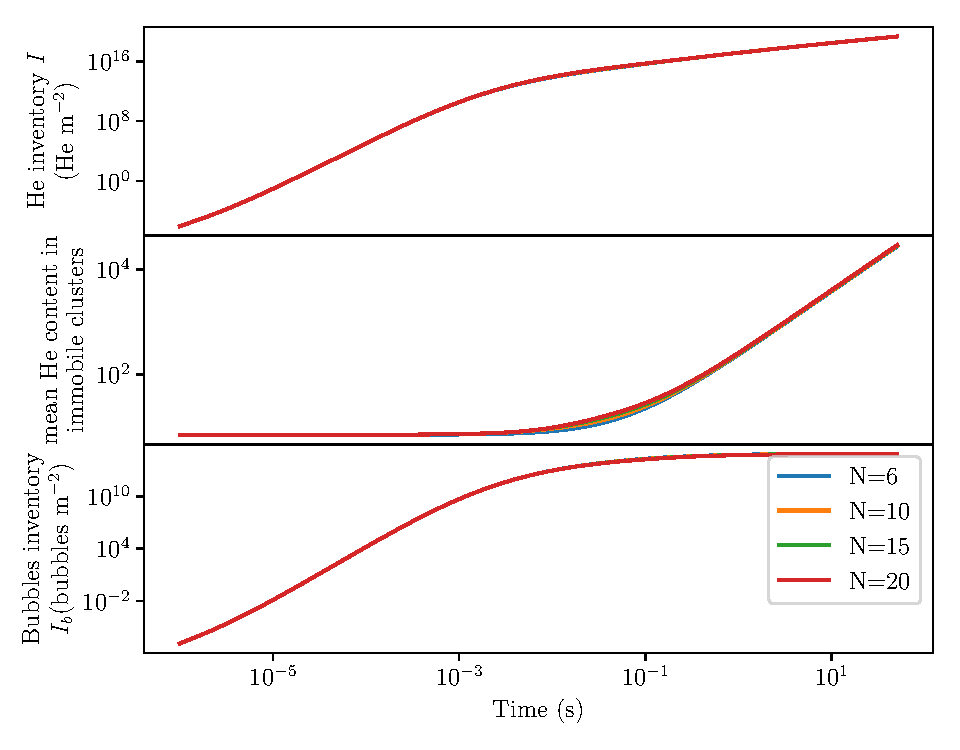
\includegraphics[width=\linewidth]{Figures/Chapter4/varying_N.pdf}
    \caption{Comparison of several quantities of interest for several values of $N$ in W exposed to \SI{100}{eV} He at \SI{e20}{m^{-2}.s^{-1}} and \SI{1000}{K}.}
    \labfig{N variation}
\end{figure}

\subsection{Comparison with experiments}

\begin{figure} [h]
    \centering
    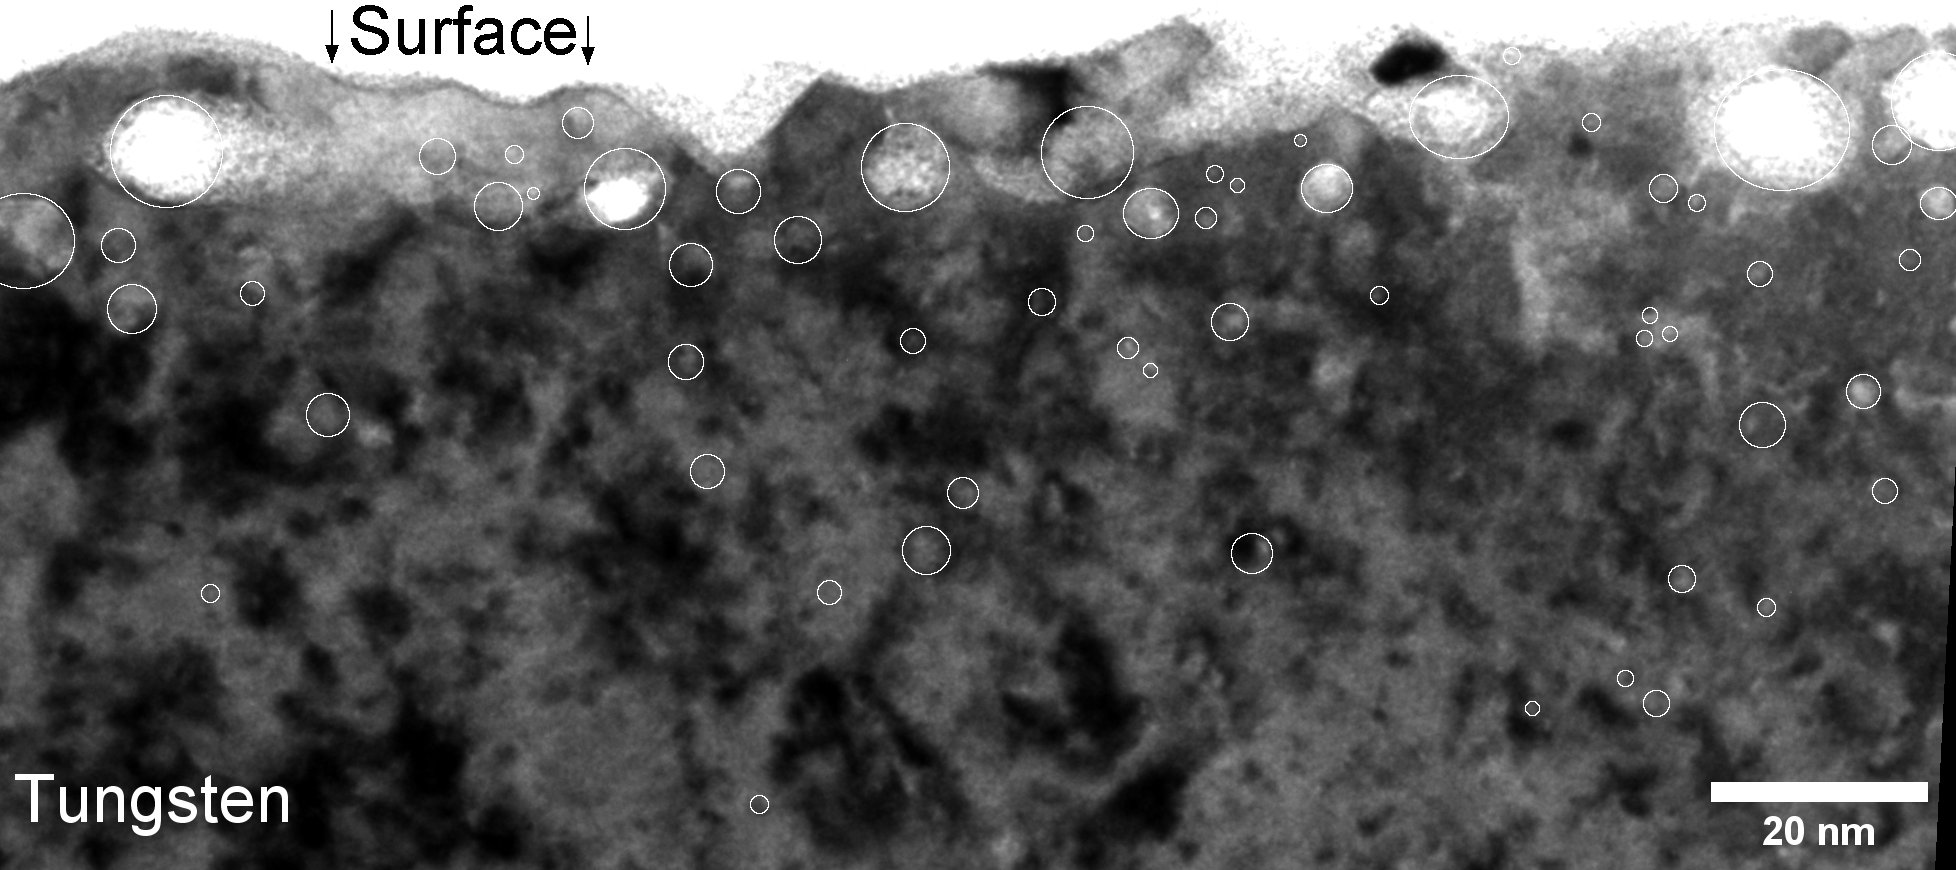
\includegraphics[width=\linewidth]{Figures/Chapter4/bubbles_tem.jpg}
    \caption{TEM images of W after exposure to \SI{75}{eV} He at \SI{2.3e22}{m^{-2}.s^{-1}} and \SI{1053}{K} for \SI{13}{s} showing bubbles that have burst, large size bubbles at the near surface and small size bubbles in the bulk.}
    \labfig{tem images}
\end{figure}

\begin{figure} [h!]
    \centering
    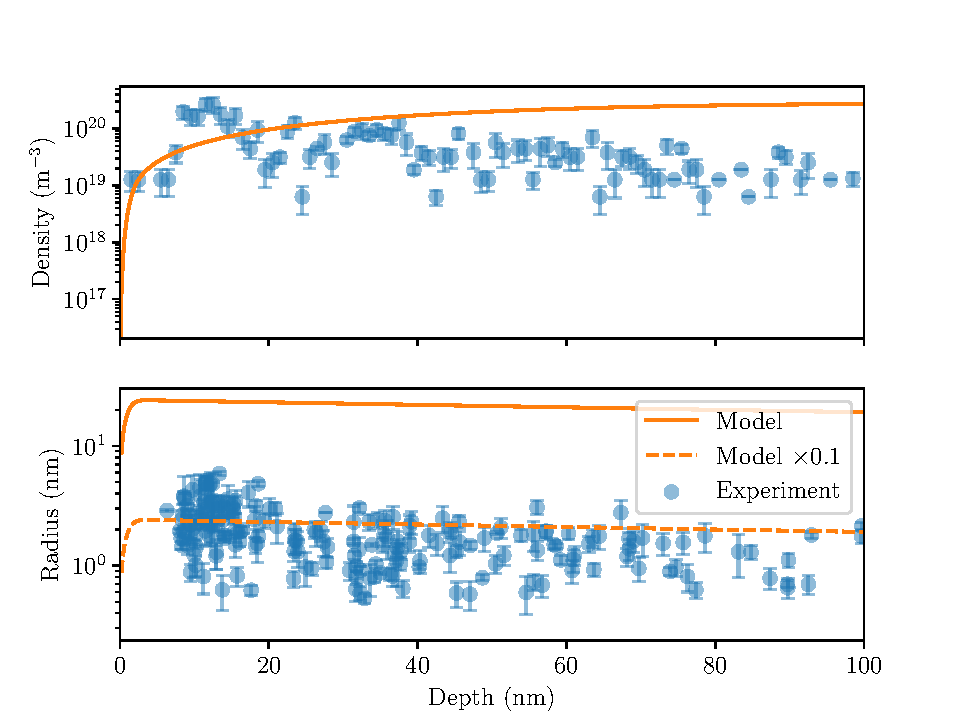
\includegraphics[width=\linewidth]{Figures/Chapter4/comparison_model_exp.pdf}
    \caption{Comparison of experimental results with simulations for W implanted with \SI{75}{eV} He at \SI{2.3e22}{m^{-2}.s^{-1}} and \SI{1053}{K} for \SI{13}{s}. Error bars correspond to the lowest and highest radius in the TEM image.}
    \labfig{exp model comparison}
\end{figure}

% He implantation experiments were performed on W and TEM (Transmission Electron Microscopy) images were produced (see \reffig{tem images}).
% W was irradiated with \SI{75}{eV} He at \SI{2.3e22}{m^{-2}.s^{-1}} and \SI{1053}{K} for \SI{13}{s}.
% Comparison of under- and over-focused TEM images allowed identification of the bubbles.
% say something about the imaging technique or the lamella...

He implantation experiments were performed on W in the linear plasma device PSI--2 \sidecite{kreter_linear_2015}.
W was irradiated with \SI{75}{eV} He at \SI{2.3e22}{m^{-2}.s^{-1}} and \SI{1053}{K} for \SI{13}{s}.
A thin lamella for cross-sectional observations was prepared using the FIB (Focused Ion Beam) technique with a Dual Beam FIB (FEI Helios 600 NanoLab).
Prior to FIB cutting, the surface of the sample was coated with a SiO layer for better contrast and then with a protective platinum layer to avoid damaging the surface during the lamella preparation.
Cross-sectional observations of the He-implanted W were performed using \gls{tem} in a TEM FEI Titan 80-300 apparatus.

A typical \gls{tem} image of the lamella is presented in \reffig{tem images}.
Comparison of under- and over-focused \gls{tem} images allowed identification of the bubbles.
Bubbles were observed up to \SI{100}{nm} with larger bubbles closer to the surface and smaller bubbles deeper in the bulk.
Open bubbles and holes at the surface were also observed suggesting bursting events occurred.
This is in accordance with what was observed in the simulations (see \reffig{profiles rb half slab}).

A procedure was developed to automate the bubble detection on \gls{tem} images using the ImageJ software \sidecite{schindelin_fiji_2012}.
The area of bubbles were computed as well as their diameter assuming a spherical shape for the bubbles.
Bubble density and size as a function of depth was therefore computed using 12 pairs of under- and over-focused \gls{tem} images.
The bubble density was found to range from \SI{7e19}{m^{-3}} to \SI{2e20}{m^{-3}} and the bubble radius ranged between \SI{1}{nm} and \SI{10}{nm} (see \reffig{exp model comparison}).
Although the resolution of the \gls{tem} is below \SI{1}{nm}, the number of bubbles with radius below \SI{2}{nm} is underestimated due to the limited contrast.

This experiment was simulated using the same exposure conditions.
The simulated bubbles density $c_b$ was found to be in accordance with the one measured experimentally.
Some discrepancies were found at the near surface.

The bubble radius ($\langle r_b \rangle$) is however overestimated by an order of magnitude compared to experimental measurements.
This could imply that the current model linking the He content to the bubble radius is overestimated and that a more accurate one is needed.
Finally, it would be worth investigating this further to determine if some saturation in the bubble size occurs and the impact of initial defects.


